\documentclass{beamer}

\usepackage{graphicx}
\usepackage{hyperref}
\DeclareGraphicsExtensions{.pdf,.png}

\usetheme{Berkeley}
\usecolortheme{seagull}
\usefonttheme{structuresmallcapsserif}

\title[HTTP]{HTTP Basics}
\author{James Condron}
\date{\today}

\begin{document}

\frame{\titlepage}

\section{Definitions}
\frame{
  \frametitle{What is http?}
  \begin{itemize}
  \item <1-> The {\tt HyperText Transfer Protocol}
  \item <2-> Uses a *request/response* model
  \item <3-> Consists of a Verb, a Path, a Version and then headers
  \item <4-> Defined at http://www.w3.org/Protocols/rfc2616/rfc2616.html
  \end{itemize}
}

\frame{
  \frametitle{HTTP/1.0 and HTTP/1.1}
  \begin{itemize}
  \item <1-> {\tt HTTP/1.0} is very basic, handled simple pages and forms
  \item <2-> {\tt HTTP/1.1} is richer and what we use today
  \item <3-> Requests made with {\tt HTTP/1.1} must include extra information
 \end{itemize}
}


\frame{
  \frametitle{TEH INTERNETZ}
  HTTP is used for two (main) things
  \begin{itemize}
  \item <1-> Passing html to a browser for human consumption
  \item <2-> Passing data via an API for computer consumption
  \end{itemize}
}

\frame{
  \frametitle{API?}
  \begin{itemize}
  \item <1-> Application Programmer's Interface
  \item <2-> Data in a format a computer can understand
  \end{itemize}
}

\section{Requests}
\frame{
  \frametitle{Everything Is Requests}
  \begin{itemize}
  \item <1-> I will be using a very simple API of my own to demonstrate HTTP
  \item <2-> And will call the API with 'curl'
  \end{itemize}
}

\subsection{Verbs}
\frame{
  \frametitle{Basics}
  \begin{itemize}
  \item <1-> The simplest three verbs to understand are *GET*, *HEAD* and *POST*
  \item <2-> These were defined in HTTP/1.0
  \item <3-> Every time you visit a website your browser performs a 'GET'
  \end{itemize}
}

\frame{
  \frametitle{Basics (Cont.)}
  \begin{figure}[h]
    \centering
    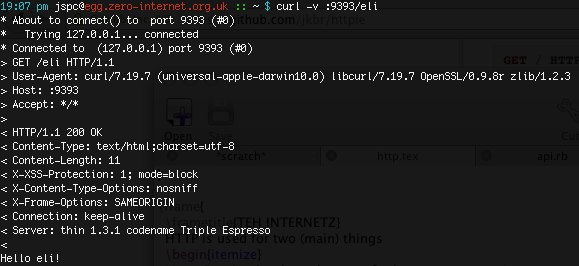
\includegraphics[width=2.5in]{img/get.png}
    \caption{GET request on '/eli'}
    \label{fig:get}
   \end{figure}
}

\frame{
  \frametitle{GET}
  \begin{itemize}
  \item <1-> First defined under {\tt HTTP/1.0}
  \item <2-> Must include the URI to query and the Host on which to do so
  \end{itemize}
}

\frame{
  \frametitle{GET (Cont.)}
  \begin{figure}[h]
    \centering
    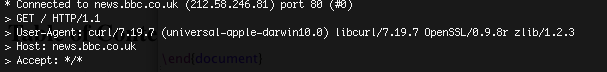
\includegraphics[width=3.5in]{img/get_req.png}
    \caption{GET request on '/'}
    \label{fig:get request full}
   \end{figure}
}

\frame{
  \frametitle{POST}
  \begin{itemize}
  \item <1-> Also first defined under {\tt HTTP/1.0}
  \item <2-> We use this to send form data
  \item <3-> It takes data in {\tt key=value} form
  \item <4-> Each pair is seperated with {\tt \&}
 \end{itemize}
}

\frame{
  \frametitle{POST (Cont.)}
  \begin{figure}[h]
    \centering
    
\includegraphics[width=3.5in]{img/post_req.png}
    \caption{POST request to '/person/me'}
    \label{fig:post request full}
   \end{figure}
}

\section{Responses}
\frame{
  \frametitle{Basics}
  \begin{itemize}
  \item <1-> Every request returns a response
  \item <2-> Usually this has some kind of data; a website or status
  \item <3-> They always have a response code
  \end{itemize}
}

\frame{
  \frametitle{Basics (Cont.)}
  \begin{figure}[h]
    \centering
    
\includegraphics[height=2.5in]{img/500_cat.jpg}
    \caption{500 Cat}
    \label{fig:500 cat}
   \end{figure}
}

\frame{
  \frametitle{1xx Response}
  \begin{itemize}
  \item <1-> Purely informational/ 'Request Received'
  \item <2-> Didn't exist in {\tt HTTP/1.0}
  \item <3-> Rarely need to use 1xx codes
  \end{itemize}
}

\frame{
  \frametitle{2xx Response}
  \begin{itemize}
  \item <1-> SUCCESS!!!!!!11111!111!!w33
  \item <2-> Generally use 200
  \item <3-> These statuses tell the requester that whatever they were trying to do worked
  \end{itemize}
}

\frame{
  \frametitle{3xx Response}
  \begin{itemize}
  \item <1-> Redirection
  \item <2-> These tell the requester that whatever it was they're looking for lives elsewhere
  \item <3-> These are important to catch: usually we want to follow redirects to get to where we want to be
  \end{itemize}
}

\frame{
  \frametitle{4xx Response}
  \begin{itemize}
  \item <1-> Client Side Error
  \item <2-> These mean the requester made a boo-boo
  \item <3-> Take {\tt 404} errors- the resource you want doesn't exist
  \item <4-> Or {\tt 403} - you're not allowed to see it
  \item <5-> {\tt 418} means ``I'm a teapot''
  \end{itemize}
}

\frame{
  \frametitle{5xx Response}
  \begin{itemize}
  \item <1-> These are *server* errors
  \item <2-> {\tt 503} errors, for example, means 'Service Unavailable'
 \end{itemize}
}

\end{document}
